\documentclass[10pt,ignorenonframetext,,aspectratio=149]{beamer}
\usefonttheme{serif} % use mainfont rather than sansfont for slide text
\setbeamertemplate{caption}[numbered]
\setbeamertemplate{caption label separator}{: }
\setbeamercolor{caption name}{fg=normal text.fg}
\usepackage{lmodern}
\usepackage{amssymb,amsmath}
\usepackage{ifxetex,ifluatex}
\usepackage{fixltx2e} % provides \textsubscript
\ifnum 0\ifxetex 1\fi\ifluatex 1\fi=0 % if pdftex
  \usepackage[T1]{fontenc}
  \usepackage[utf8]{inputenc}
\else % if luatex or xelatex
  \ifxetex
    \usepackage{mathspec}
  \else
    \usepackage{fontspec}
  \fi
  \defaultfontfeatures{Ligatures=TeX,Scale=MatchLowercase}
  \newcommand{\euro}{€}
    \setmainfont[]{Open Sans}
\fi
% use upquote if available, for straight quotes in verbatim environments
\IfFileExists{upquote.sty}{\usepackage{upquote}}{}
% use microtype if available
\IfFileExists{microtype.sty}{%
\usepackage{microtype}
\UseMicrotypeSet[protrusion]{basicmath} % disable protrusion for tt fonts
}{}
\usepackage{graphicx,grffile}
\makeatletter
\def\maxwidth{\ifdim\Gin@nat@width>\linewidth\linewidth\else\Gin@nat@width\fi}
\def\maxheight{\ifdim\Gin@nat@height>\textheight0.8\textheight\else\Gin@nat@height\fi}
\makeatother
% Scale images if necessary, so that they will not overflow the page
% margins by default, and it is still possible to overwrite the defaults
% using explicit options in \includegraphics[width, height, ...]{}
\setkeys{Gin}{width=\maxwidth,height=\maxheight,keepaspectratio}

% Comment these out if you don't want a slide with just the
% part/section/subsection/subsubsection title:
\AtBeginPart{
  \let\insertpartnumber\relax
  \let\partname\relax
  \frame{\partpage}
}
\AtBeginSection{
  \let\insertsectionnumber\relax
  \let\sectionname\relax
  \frame{\sectionpage}
}
\AtBeginSubsection{
  \let\insertsubsectionnumber\relax
  \let\subsectionname\relax
  \frame{\subsectionpage}
}

\setlength{\emergencystretch}{3em}  % prevent overfull lines
\providecommand{\tightlist}{%
  \setlength{\itemsep}{0pt}\setlength{\parskip}{0pt}}
\setcounter{secnumdepth}{0}

\title{The Least Squares Linear Regression Model}
\author{Henrique Veras}
\date{}

%% Here's everything I added.
%%--------------------------

\usepackage{graphicx}
\usepackage{rotating}
%\setbeamertemplate{caption}[numbered]
\usepackage{hyperref}
\usepackage{caption}
\usepackage[normalem]{ulem}
%\mode<presentation>
\usepackage{wasysym}
%\usepackage{amsmath}


% Get rid of navigation symbols.
%-------------------------------
\setbeamertemplate{navigation symbols}{}

% Optional institute tags and titlegraphic.
% Do feel free to change the titlegraphic if you don't want it as a Markdown field.
%----------------------------------------------------------------------------------
\institute{PIMES/UFPE}

% \titlegraphic{\includegraphics[width=0.3\paperwidth]{\string~/Dropbox/teaching/clemson-academic.png}} % <-- if you want to know what this looks like without it as a Markdown field. 
% -----------------------------------------------------------------------------------------------------


% Some additional title page adjustments.
%----------------------------------------
\setbeamertemplate{title page}[empty]
%\date{}
\setbeamerfont{subtitle}{size=\small}

\setbeamercovered{transparent}

% Some optional colors. Change or add as you see fit.
%---------------------------------------------------
\definecolor{clemsonpurple}{HTML}{522D80}
 \definecolor{clemsonorange}{HTML}{F66733}
\definecolor{uiucblue}{HTML}{003C7D}
\definecolor{uiucorange}{HTML}{F47F24}


% Some optional color adjustments to Beamer. Change as you see fit.
%------------------------------------------------------------------
\setbeamercolor{frametitle}{fg=clemsonpurple,bg=white}
\setbeamercolor{title}{fg=clemsonpurple,bg=white}
\setbeamercolor{local structure}{fg=clemsonpurple}
\setbeamercolor{section in toc}{fg=clemsonpurple,bg=white}
% \setbeamercolor{subsection in toc}{fg=clemsonorange,bg=white}
\setbeamercolor{footline}{fg=clemsonpurple!50, bg=white}
\setbeamercolor{block title}{fg=clemsonorange,bg=white}


\let\Tiny=\tiny


% Sections and subsections should not get their own damn slide.
%--------------------------------------------------------------
\AtBeginPart{}
\AtBeginSection{}
\AtBeginSubsection{}
\AtBeginSubsubsection{}

% Suppress some of Markdown's weird default vertical spacing.
%------------------------------------------------------------
\setlength{\emergencystretch}{0em}  % prevent overfull lines
\setlength{\parskip}{0pt}


% Allow for those simple two-tone footlines I like. 
% Edit the colors as you see fit.
%--------------------------------------------------
\defbeamertemplate*{footline}{my footline}{%
    \ifnum\insertpagenumber=1
    \hbox{%
        \begin{beamercolorbox}[wd=\paperwidth,ht=.8ex,dp=1ex,center]{}%
      % empty environment to raise height
        \end{beamercolorbox}%
    }%
    \vskip0pt%
    \else%
        \Tiny{%
            \hfill%
		\vspace*{1pt}%
            \insertframenumber/\inserttotalframenumber \hspace*{0.1cm}%
            \newline%
            \color{clemsonpurple}{\rule{\paperwidth}{0.4mm}}\newline%
            \color{clemsonorange}{\rule{\paperwidth}{.4mm}}%
        }%
    \fi%
}

% Various cosmetic things, though I must confess I forget what exactly these do and why I included them.
%-------------------------------------------------------------------------------------------------------
\setbeamercolor{structure}{fg=blue}
\setbeamercolor{local structure}{parent=structure}
\setbeamercolor{item projected}{parent=item,use=item,fg=clemsonpurple,bg=white}
\setbeamercolor{enumerate item}{parent=item}

% Adjust some item elements. More cosmetic things.
%-------------------------------------------------
\setbeamertemplate{itemize item}{\color{clemsonpurple}$\bullet$}
\setbeamertemplate{itemize subitem}{\color{clemsonpurple}\scriptsize{$\bullet$}}
\setbeamertemplate{itemize/enumerate body end}{\vspace{.6\baselineskip}} % So I'm less inclined to use \medskip and \bigskip in Markdown.

% Automatically center images
% ---------------------------
% Note: this is for ![](image.png) images
% Use "fig.align = "center" for R chunks

\usepackage{etoolbox}

\AtBeginDocument{%
  \letcs\oig{@orig\string\includegraphics}%
  \renewcommand<>\includegraphics[2][]{%
    \only#3{%
      {\centering\oig[{#1}]{#2}\par}%
    }%
  }%
}

% I think I've moved to xelatex now. Here's some stuff for that.
% --------------------------------------------------------------
% I could customize/generalize this more but the truth is it works for my circumstances.

\ifxetex
\setbeamerfont{title}{family=\fontspec{Titillium Web}}
\setbeamerfont{frametitle}{family=\fontspec{Titillium Web}}
\usepackage[font=small,skip=0pt]{caption}
 \else
 \fi

% Okay, and begin the actual document...

\begin{document}
\frame{\titlepage}

\hypertarget{econometrics}{%
\section{Econometrics}\label{econometrics}}

\hypertarget{intro}{%
\subsection{Intro}\label{intro}}

\begin{frame}{Introduction}
\protect\hypertarget{introduction}{}
Model builders are oftern interested in understanding the
\emph{conditional variation} of one variable relative to others rather
than their \emph{joint probability}

\vfill

Question: What feature of the conditional probability distribution are
we interested in?

\vfill

Usually, the expected value \(E[y|x]\), but sometimes might be:

~~~~~~ Conditional median or other quantiles of the distribution (20th
percentile,

~~~~~~ 5th percentile, etc), variance \vfill

Linear regression deals with \textbf{conditional mean}
\end{frame}

\hypertarget{the-linear-regression-model}{%
\subsection{The Linear Regression
Model}\label{the-linear-regression-model}}

\begin{frame}{The Linear Regression Model}
\protect\hypertarget{the-linear-regression-model-1}{}
\(\mathbf{y}=f(\textbf{x}_1, \textbf{x}_2, \cdots, \textbf{x}_k)+\varepsilon\),
where \(\varepsilon\) is called the \textbf{disturbance} term.

\vfill

Our \textbf{theory} will specify the population regression equation
\(f(\textbf{x}_1, \textbf{x}_2, \cdots, \textbf{x}_k)\), which
encompasses its format and the variables that matter.

\vfill
\end{frame}

\hypertarget{assumptions-of-the-linear-regression-model}{%
\subsection{Assumptions of the Linear Regression
Model}\label{assumptions-of-the-linear-regression-model}}

\begin{frame}{Assumptions of the Linear Regression Model}
\protect\hypertarget{assumptions-of-the-linear-regression-model-1}{}
The linear regression model consists of a set of assumptions about how a
data set will be produced by an underlying ''data generating process.''

\vfill

\textbf{Assumption A1}: The model specifies a linear relationship
between \(y\) and \(\textbf{x}_1,\cdots, \textbf{x}_k\):

\[\mathbf{y}=\textbf{x}_1\mathbf{\beta}_1+\textbf{x}_2\mathbf{\beta}_2+\cdots+\textbf{x}_k\mathbf{\beta}_k+\mathbf{\varepsilon}\]

\vfill

Notice that the assumption is about the linearity in the parameters
rather than in the \(\mathbf{x}\)'s.
\end{frame}

\begin{frame}{Linearity of the Regression Model}
\protect\hypertarget{linearity-of-the-regression-model}{}
Each observation of a given data set looks like

\[y_1=\beta_1 x_{11}+\beta_2x_{21}+\cdots\beta_kx_{k1}+\varepsilon_1\]

\[y_2=\beta_1 x_{12}+\beta_2x_{22}+\cdots\beta_kx_{k2}+\varepsilon_1\]

\[\vdots\]

\[y_n=\beta_1 x_{1n}+\beta_2x_{2n}+\cdots\beta_kx_{kn}+\varepsilon_1\]
\end{frame}

\begin{frame}{Linearity of the Regression Model}
\protect\hypertarget{linearity-of-the-regression-model-1}{}
In Matrix form:

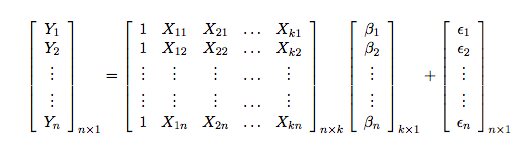
\includegraphics{/Users/henriquefonseca/Desktop/temp/Rmarkdown-practice/henriqueveras.github.io/files/Econometrics/Lecture Notes/2/matrix2.png}

\[\textbf{y}=\textbf{X}\mathbf{\beta}+\mathbf{\varepsilon}\]
\end{frame}

\begin{frame}{Ful Rank}
\protect\hypertarget{ful-rank}{}
\textbf{Assumption A2}: The columns of \(X\) are linearly independent
and there are at least \(k\) observations.

\vfill

Assumption A2 states that there are no linear relationships among the
variables.

\vfill

Here's an example of a model that cannot be estimated, although we might
be interested in quantifying each of the coefficients: the determinants
of Monet's prices:

\[\ln \text{Price} = \beta_1 \ln \text{Size} + \beta_2 \ln \text{Aspect Ratio} + \beta_3  \ln \text{Height}+\varepsilon\]

where \(\text{Size}=\text{Width}\times\text{Height}\) and
\(\text{Aspect Ratio}=Width/Height\)
\end{frame}

\begin{frame}{Regression}
\protect\hypertarget{regression}{}
\textbf{Assumption A3}: The disturbance is assumed to have conditional
expected value zero at every observation:
\(E(\mathbf{\varepsilon}|\mathbf{X})=0\)

\vfill

No value of \(\mathbf{X}\) conveys any information about
\(\varepsilon\). We assume that \(\varepsilon_i\)'s are purely random
draws from a population.

\vfill

Moreover, we assume
\(E[\varepsilon_i|\varepsilon_1, \cdots, \varepsilon_{i-1}, \varepsilon_{i+1}, \cdots, \varepsilon_n ]=0\).

\vfill

Notice that by the \textbf{Law of Iterated Expectations}:
\[E[\varepsilon_i]=E_X[E[\varepsilon_i|\mathbf{X}]]=E_X[0]=0\]

\vfill
\end{frame}

\begin{frame}{Regression}
\protect\hypertarget{regression-1}{}
Point to note:
\(E[\varepsilon|\mathbf{X}]=0 \Rightarrow Cov(\mathbf{X},\varepsilon)=0\).
But the converse is not true: \(E[\varepsilon]=0\) \textbf{does not}
imply that \(E[\varepsilon|\mathbf{X}]=0\).

\vfill

Accordingly, \(E[\mathbf{y}|\mathbf{X}]=\mathbf{X}\mathbf{\beta}\).

\vfill

Assumptions \textbf{A1} and \textbf{A3} comprise the \emph{linear
regression model}.

\vfill

What if \(E[\mathbf{\varepsilon}]\neq0\)?
\end{frame}

\begin{frame}{}
\protect\hypertarget{section}{}
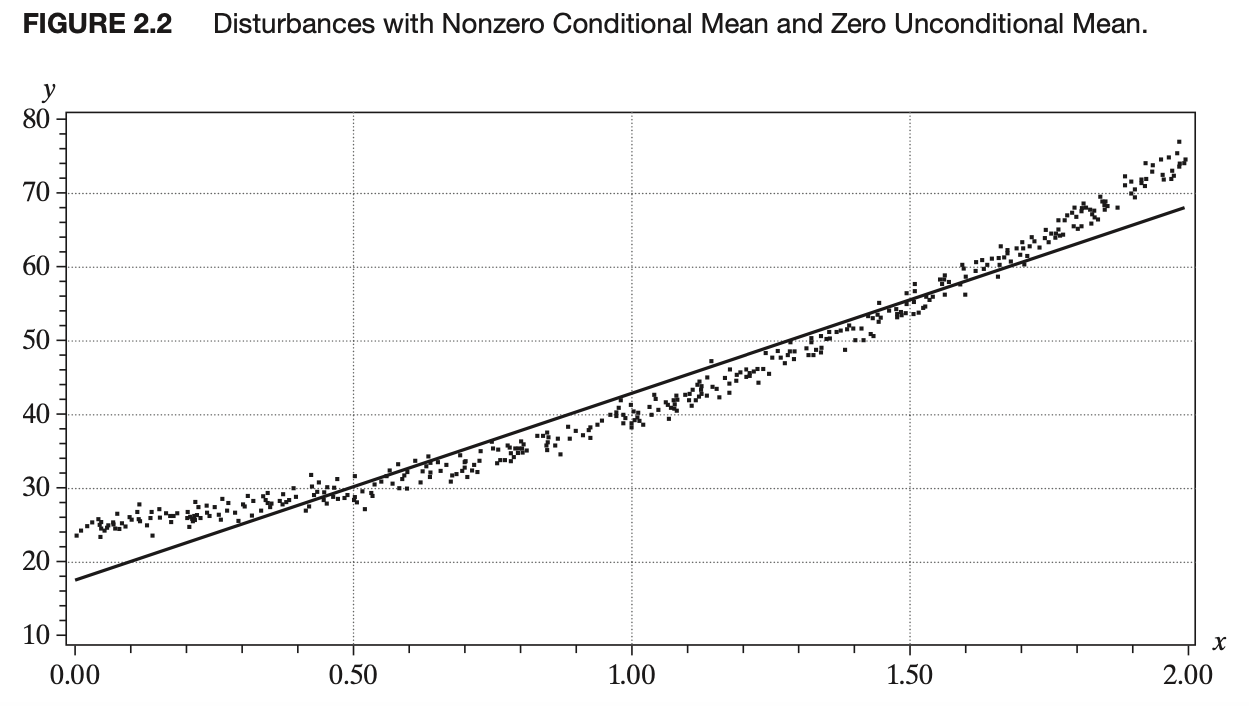
\includegraphics{/Users/henriquefonseca/Desktop/temp/Rmarkdown-practice/henriqueveras.github.io/files/Econometrics/Lecture Notes/2/example_2.2.png}
\end{frame}

\begin{frame}{Regression}
\protect\hypertarget{regression-2}{}
Assumption \textbf{A3} is called the \textbf{exogeneity} assumption and
it yields \(E[\mathbf{y}]=\mathbf{X}\mathbf{\beta}\).

\vfill

Whenever \(E(\mathbf{\varepsilon}|x)\neq 0\), we say that \(x\) is
\textbf{endogenous} to the model. One way that this can happen is when
we leave out a variable that matters for the relationship.

\vfill

Suppose the DGP of a given relationship is given by
\[Income=\gamma_1+\gamma_2 educ+\gamma_3 age +u\] but we estimate the
model \[Income=\gamma_1+\gamma_2 educ +\varepsilon\]

\vfill

How do we show that \textbf{A3} is not satisfied?
\end{frame}

\begin{frame}{Homoskedasticity and Nonautocorrelated Disturbances}
\protect\hypertarget{homoskedasticity-and-nonautocorrelated-disturbances}{}
\textbf{Assumption A4}:
\(E[{\varepsilon\varepsilon'|\mathbf{X}}]=\sigma^2\mathbf{I}\)

\vfill

Also, notice that
\(Var[\varepsilon]=E[Var(\varepsilon|\mathbf{X})]+Var[E(\varepsilon|\mathbf{X})]=\sigma^2\mathbf{I}\)
\end{frame}

\begin{frame}{Data Generating Process for the Regressors}
\protect\hypertarget{data-generating-process-for-the-regressors}{}
\textbf{Assumption A5}: \(\mathbf{X}\) may be fixed or random.

\vfill

Fixed \(\mathbf{X}\): Experimental designs, whereby the researcher fixes
the values of \(\mathbf{X}\) to find \(\mathbf{y}\).

\vfill

Random \(\mathbf{X}\): Observational studies. However, some columns of
the \(\mathbf{X}\) can be fixed, such as indicator variables for a given
time period or time trends.
\end{frame}

\begin{frame}{Normality}
\protect\hypertarget{normality}{}
\textbf{Assumption A6}:
\(\varepsilon|\mathbf{X} \sim N(\mathbf{0},\sigma^2\mathbf{I})\)

\vfill

This assumption is useful for hypothesis testing and constructing
confidence intervals but might not be needed as the Central Limit
Theorem applies to sufficiently large data.
\end{frame}

\begin{frame}{Visual Summary of the Assumptions}
\protect\hypertarget{visual-summary-of-the-assumptions}{}
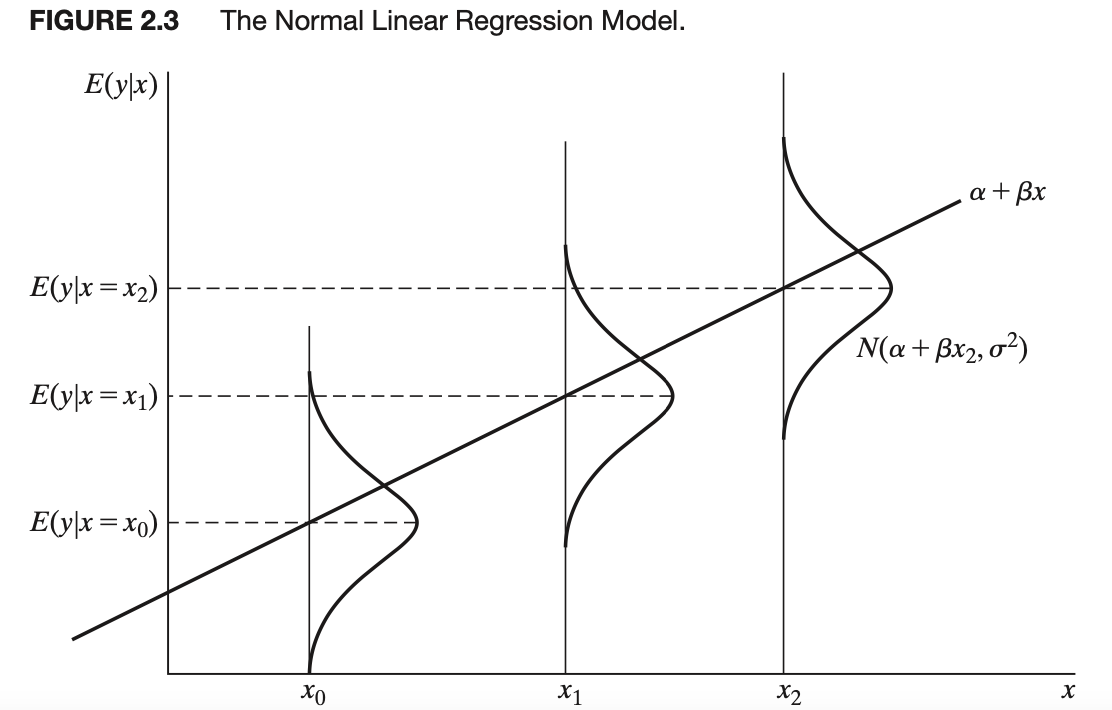
\includegraphics{/Users/henriquefonseca/Desktop/temp/Rmarkdown-practice/henriqueveras.github.io/files/Econometrics/Lecture Notes/2/figure_2.3.png}
\end{frame}

\hypertarget{computation-of-the-least-squares-regression}{%
\subsection{Computation of the Least Squares
Regression}\label{computation-of-the-least-squares-regression}}

\begin{frame}{Computational Aspects of the Least Squares Regression}
\protect\hypertarget{computational-aspects-of-the-least-squares-regression}{}
Let's now consider the algebraic problem of choosing a vector
\(\mathbf{b}\) so that the fitted line \(\mathbf{x}_i'\mathbf{b}\) is
\emph{close} to the data.

\vfill

We need to specify what do we mean by \emph{close} to the data (the
fitting criterion).

\vfill

Usually, the fitting criterion is the \emph{Least Squares} method:
minimizing the sum of the squared deviations from the mean.

\vfill

Crucial feature: LS regression provides us a device for ``holding other
things constant''.

\vfill
\end{frame}

\begin{frame}{The LS Population and Sample Models}
\protect\hypertarget{the-ls-population-and-sample-models}{}
Recall the population regression model:
\(E[y_i|\mathbf{x}_i]=\mathbf{x}_i'\beta\)

\vfill

We aim to find an estimate \(\hat{y_i}=\mathbf{x}_i'\mathbf{b}\)

\vfill

Define the \emph{residuals} from the estimated regression as
\[e_i=y_i-\mathbf{x}'_ib\]

\vfill

Notice that \(y_i=\mathbf{x}_i'\beta+\varepsilon_i=\mathbf{x}_i'b+e_i\)
\vfill
\end{frame}

\begin{frame}{The LS Coefficient Vector}
\protect\hypertarget{the-ls-coefficient-vector}{}
The Least Squares criterion requires us to minimize
\[\sum_{i=1}^n{e_i^2}=\sum_{i=1}^n{(y_i-\mathbf{x}_i'b)^2}\]

\vfill

In matrix terms, we minimize

\[S(\mathbf{b})=\mathbf{e}'\mathbf{e}=(\mathbf{y}-\mathbf{X}\mathbf{b})'(\mathbf{y}-\mathbf{X}\mathbf{b})\]

\vfill

Expanding, we have
\[S(\mathbf{b})=\mathbf{y}'\mathbf{y}-2\mathbf{y}'\mathbf{X}\mathbf{b}+\mathbf{b}'\mathbf{X}'\mathbf{X}\mathbf{b}\]

\vfill
\end{frame}

\begin{frame}{The LS Coefficient Vector}
\protect\hypertarget{the-ls-coefficient-vector-1}{}
The necessary condition for a minimum is
\[\frac{\partial S(\mathbf{b})}{\partial \mathbf{b}}=-2\mathbf{X}'\mathbf{y}+2\mathbf{X}'\mathbf{X}\mathbf{b}=\mathbf{0}\]
\[\mathbf{X}'\mathbf{X}\mathbf{b}=\mathbf{X}'\mathbf{y}\]

\vfill

From \textbf{A2}, we know that \(\mathbf{X}\) has full rank, which
guarantees the existence of its inverse. Then, pre-multiplying both
sides by \((\mathbf{X}'\mathbf{X})^{-1}\):

\[b_0=(\mathbf{X}'\mathbf{X})^{-1}\mathbf{X}'\mathbf{y}\]

\vfill

For the solution \(b_0\) to minimize the sum of the squared residuals,
the matrix
\(\frac{\partial^2 S(\mathbf{b})}{\partial \mathbf{b}^2}=2\mathbf{X}'\mathbf{X}\)
must be positive definite.
\end{frame}

\begin{frame}{Algebraic Aspects of the LS Solution}
\protect\hypertarget{algebraic-aspects-of-the-ls-solution}{}
We have
\[\mathbf{X}'\mathbf{X}\mathbf{b}-\mathbf{X}'\mathbf{y}=-\mathbf{X}'(\mathbf{y}-\mathbf{X}\mathbf{b})=-\mathbf{X}'\mathbf{e}=\mathbf{0}\]

\vfill

Hence, for every column of \(\mathbf{X}\),
\(\mathbf{x}_k'\mathbf{e}=0\).

\vfill

Denote the first row \(\mathbf{X}\) as
\(\mathbf{x}_1\equiv \mathbf{i}\), two implications follow:

\begin{enumerate}
\tightlist
\item
  The LS residuals sum to zero.
\item
  The regression hyperplane passes through the point of means of the
  data.
\end{enumerate}

\vfill
\end{frame}

\begin{frame}{Projection}
\protect\hypertarget{projection}{}
Recall the LS residuals: \[\mathbf{e}=\mathbf{y}-\mathbf{Xb}\]

\vfill

Inserting \(\mathbf{b}_0\), we have
\[\mathbf{e}=\mathbf{y}-\mathbf{X}(\mathbf{X}'\mathbf{X})^{-1}\mathbf{X}'\mathbf{y}=(\mathbf{I}-\mathbf{X}(\mathbf{X}'\mathbf{X})^{-1}\mathbf{X}')\mathbf{y}=\mathbf{M}\mathbf{y}\]

\vfill

The matrix \(\mathbf{M}\) is called the ``\emph{residual maker}'':

\vfill

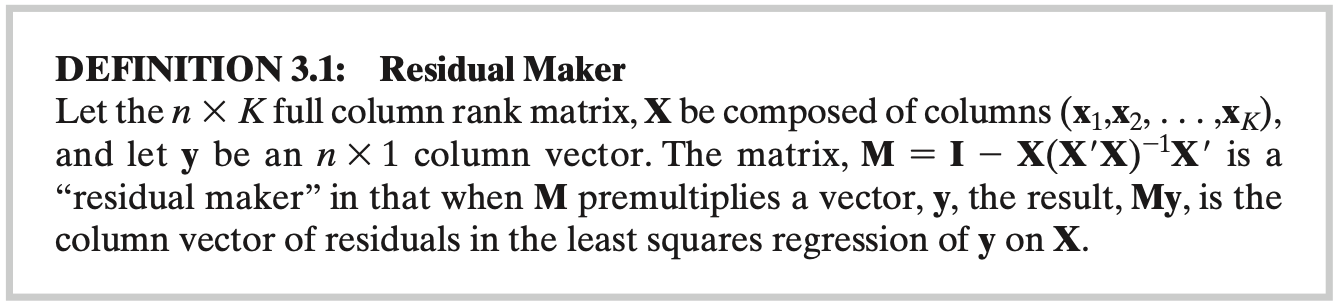
\includegraphics{/Users/henriquefonseca/Desktop/temp/Rmarkdown-practice/henriqueveras.github.io/files/Econometrics/Lecture Notes/2/definition_3.1.png}
\end{frame}

\begin{frame}{The Residual Maker}
\protect\hypertarget{the-residual-maker}{}
Properties of the matrix M:

\begin{enumerate}
\tightlist
\item
  M is symmetric
\item
  M is idempotent
\item
  \(\mathbf{MX}=\mathbf{0}\) (why?)
\end{enumerate}
\end{frame}

\begin{frame}{The Projection Matrix}
\protect\hypertarget{the-projection-matrix}{}
Now let
\[\hat{\mathbf{y}}=\mathbf{y}-\mathbf{e}=\mathbf{I}\mathbf{y}-\mathbf{My}=(\mathbf{I}-\mathbf{M})\mathbf{y}\]

\vfill

Thus,

\[\hat{\mathbf{y}}=\mathbf{X}(\mathbf{X}'\mathbf{X})^{-1}\mathbf{X}'\mathbf{y}=\mathbf{Py}\]

\vfill

P is called a \emph{projection} matrix: If a vector \(\mathbf{y}\) is
pre-multiplied by \(\mathbf{P}\), the result is the fitted values in the
LS regression of \(\mathbf{y}\) on \(\mathbf{X}\).

\vfill
\end{frame}

\begin{frame}{The Projection Matrix}
\protect\hypertarget{the-projection-matrix-1}{}
Properties of \(\mathbf{P}\):

\begin{enumerate}
\tightlist
\item
  \(\mathbf{P}\) is symmetric
\item
  \(\mathbf{P}\) is idempotent
\item
  \(\mathbf{P}\mathbf{X}=\mathbf{X}\)
\end{enumerate}

\vfill

Moreover, notice that \(\mathbf{P}\) and \(\mathbf{M}\) are orthogonal:
\(\mathbf{P}\mathbf{M}=\mathbf{M}\mathbf{P}=\mathbf{0}\)

\vfill

Therefore, the LS regression partitions the vector \(\mathbf{y}\) into
two \textbf{orthogonal} parts:
\[\mathbf{y}=\mathbf{P}\mathbf{y}+\mathbf{M}\mathbf{y}= \text{Projection}+\text{Residuals}\]
\end{frame}

\begin{frame}{}
\protect\hypertarget{section-1}{}
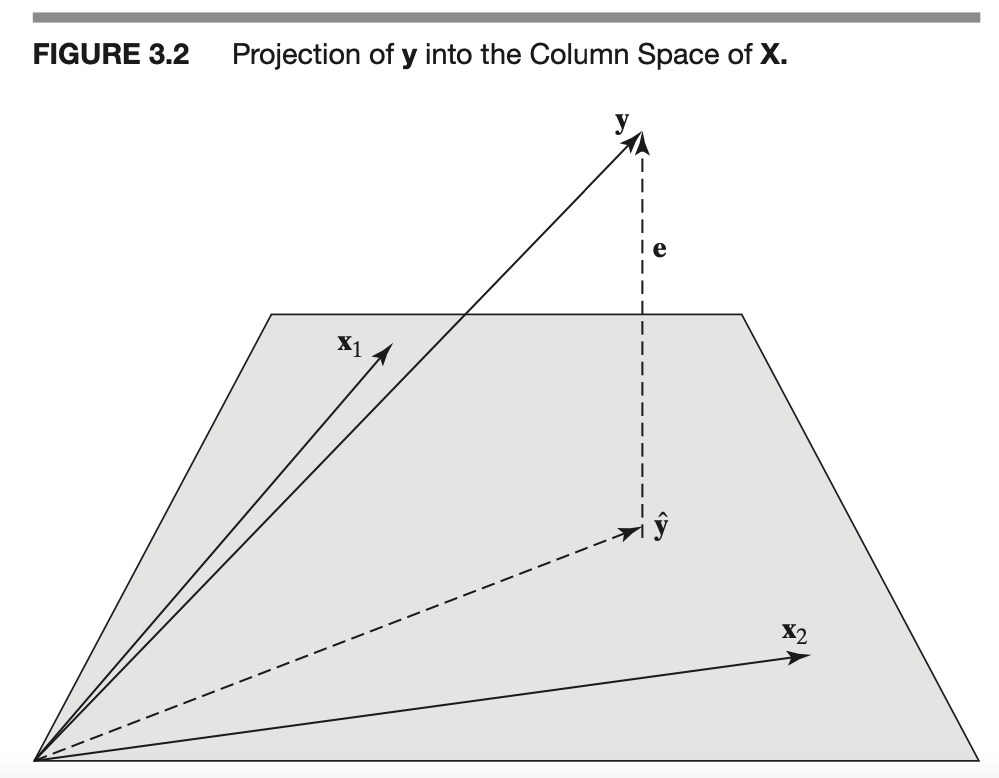
\includegraphics{/Users/henriquefonseca/Desktop/temp/Rmarkdown-practice/henriqueveras.github.io/files/Econometrics/Lecture Notes/2/figure_3.2.png}
\end{frame}

\hypertarget{partitioning-and-partial-regressions}{%
\subsection{Partitioning and Partial
Regressions}\label{partitioning-and-partial-regressions}}

\begin{frame}{Partitioning and Partial Regressions}
In some situations, we are only interested in a subset of the full set
of variables in \(\mathbf{X}\). The remaining variables are added to the
model as ``controls''.

~~~~~~ Recall the returns to education example.

\vfill

Suppose we have

\[\mathbf{y}=\mathbf{X}\mathbf{\beta}+\mathbf{\varepsilon}=\mathbf{X}_1\mathbf{\beta_1}+\mathbf{X}_2\mathbf{\beta}_2+\varepsilon\]

How can we find the algebraic solution for \(\mathbf{b}_2\)? That is,
what is the LS estimator of a given subset of parameters in
\(\mathbf{\beta}\)?
\end{frame}

\begin{frame}{Partial Regressions}
\protect\hypertarget{partial-regressions}{}
Set up the \textbf{normal} equations:

\[\begin{bmatrix} 
    \mathbf{X}_1'\mathbf{X}_1 & \mathbf{X}_1'\mathbf{X}_2 \\
    \mathbf{X}_2'\mathbf{X}_1 & \mathbf{X}_2'\mathbf{X}_2 \\
    \end{bmatrix}
%
    \begin{bmatrix} 
    \mathbf{b}_1   \\
\mathbf{b}_2  \\
    \end{bmatrix} = 
%   
    \begin{bmatrix} 
    \mathbf{X}_1'\mathbf{y}   \\
\mathbf{X}_2'\mathbf{y}  \\
    \end{bmatrix}\]

\vfill

Solving the system above for \(\mathbf{b}_1\) yields

\[\mathbf{b}_1=(\mathbf{X}_1'\mathbf{X}_1)^{-1}\mathbf{X}_1')(\mathbf{y}-\mathbf{X}_2\mathbf{b}_2)\]
\end{frame}

\begin{frame}{Partial Regressions}
\protect\hypertarget{partial-regressions-1}{}
Suppose that \(\mathbf{X}_1'\mathbf{X}_2=0\). (what does this mean?)

\vfill

For this special case, the theorem below states that \(\mathbf{b}_1\)
can be obtained by regressing \(\mathbf{y}\) on \(\mathbf{X}_1\) only.
Likewise, \(\mathbf{b}_2\) can be obtained by regressing \(\mathbf{y}\)
on \(\mathbf{X}_2\) only.

\vfill

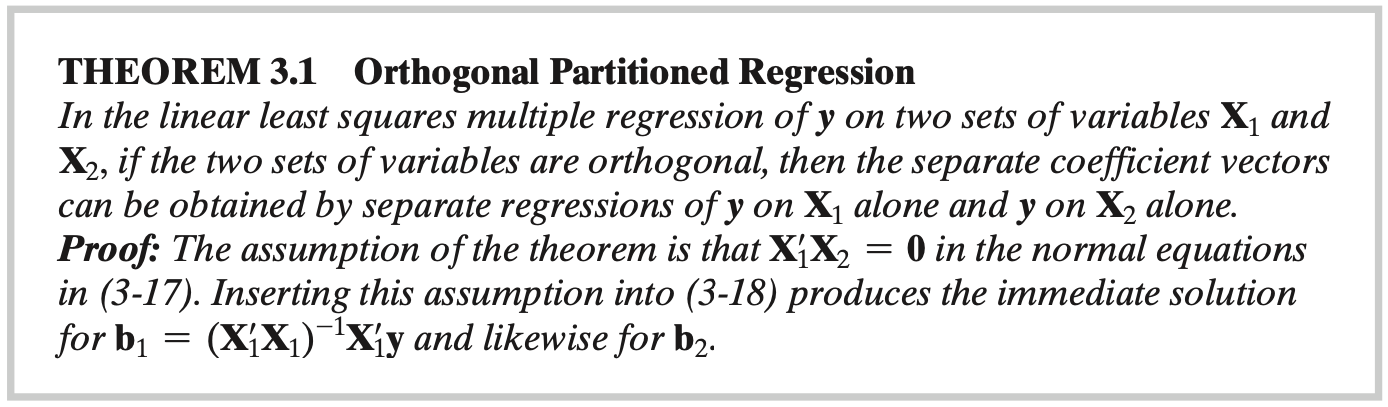
\includegraphics{/Users/henriquefonseca/Desktop/temp/Rmarkdown-practice/henriqueveras.github.io/files/Econometrics/Lecture Notes/2/theorem_3.1.png}
\end{frame}

\begin{frame}{The FWL Theorem}
\protect\hypertarget{the-fwl-theorem}{}
For the general case, in which \(\mathbf{X}_1\) and \(\mathbf{X}_2\)
might not be orthogonal, the following theorem provides the more general
solution:

\vfill

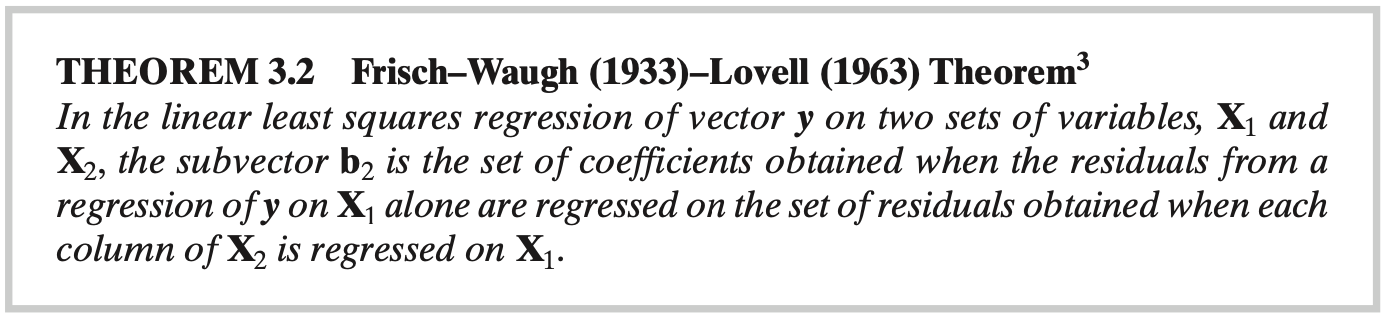
\includegraphics{/Users/henriquefonseca/Desktop/temp/Rmarkdown-practice/henriqueveras.github.io/files/Econometrics/Lecture Notes/2/theorem_3.2.png}
\end{frame}

\begin{frame}{The FWL Theorem}
\protect\hypertarget{the-fwl-theorem-1}{}
We can represent \(\mathbf{b}_2\) as
\[\mathbf{b}_2=(\mathbf{X}_2^{*'}\mathbf{X}_2^{*})^{-1}\mathbf{X}_2^{*'}\mathbf{y}^{*}\]

\vfill

where \(\mathbf{X}_2^{*}=\mathbf{M}_1\mathbf{X}_2\) and
\(\mathbf{y}^*=\mathbf{M}_1\mathbf{y}\).

\vfill

Two questions:

\begin{enumerate}
\tightlist
\item
  What is \(\mathbf{M}_1\mathbf{X}_2\)?
\item
  What is \(\mathbf{M}_1\mathbf{y}\)?
\end{enumerate}

\vfill
\end{frame}

\hypertarget{the-fwl-theorem-2}{%
\subsection{The FWL Theorem}\label{the-fwl-theorem-2}}

\begin{frame}{The FWL Theorem}
A special case of the FWL theorem is when we are interested in the
computation of a single coefficient.

\vfill

Consider the regression of \(\mathbf{y}\) on a set of variables
\(\mathbf{X}\) and an additional variable \(z\). Denote the coefficients
\(\mathbf{b}\) and \(c\), respectively.

\vfill

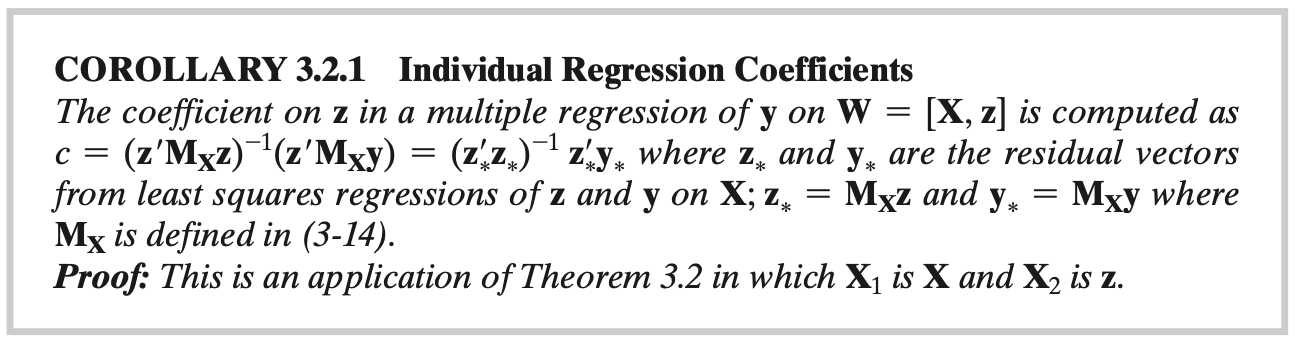
\includegraphics{/Users/henriquefonseca/Desktop/temp/Rmarkdown-practice/henriqueveras.github.io/files/Econometrics/Lecture Notes/2/corollary_3.2.1.png}
\end{frame}

\begin{frame}{The FWL Theorem}
\protect\hypertarget{the-fwl-theorem-3}{}
Example: Suppose we are interested again in the returns to education
equation
\[Income=\beta_1+\beta_2 educ + \beta_3 age + \beta_4 age^2+\varepsilon\]

\vfill

To find \(b_1\):

\begin{enumerate}
\tightlist
\item
  Regress \(Income\) on \(age\) and \(age^2\) and obtain residuals
  \(r_1\)
\item
  Regress \(educ\) on \(age\) and \(age^2\) and obtain residuals \(r_2\)
\item
  Regress \(r_1\) on \(r_2\) and find slope coefficient \(b_1\).
\end{enumerate}
\end{frame}

\begin{frame}{Regression with a constant term}
\protect\hypertarget{regression-with-a-constant-term}{}
Consider now the partition in which \(\mathbf{X}_1=\mathbf{i}\) and
\(\mathbf{X}_2\) is the set of variables in the regression.

\vfill

Take a given column \(\mathbf{x}\) of \(\mathbf{X}_2\). According to the
FWL theorem,

\[\mathbf{x}^*=\mathbf{M}_1\mathbf{x}\] \vfill

This yields

\[\mathbf{x}^*=\mathbf{x}-\mathbf{i}\mathbf{\bar{x}}\] \vfill
\end{frame}

\begin{frame}{Regression with a constant term}
\protect\hypertarget{regression-with-a-constant-term-1}{}
The result above says that the residuals in the regression of the
columns of \(\mathbf{X}_2\) on a constant term are deviations from the
sample mean.

\vfill

Therefore, each column of \(\mathbf{M}_1\mathbf{X}_2\) is the original
variable, now in the form of deviations from the mean. This general
result is summarized in the following corollary.

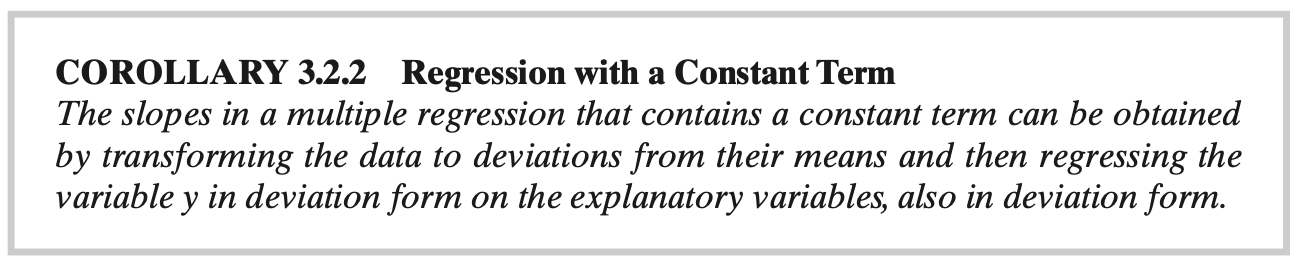
\includegraphics{/Users/henriquefonseca/Desktop/temp/Rmarkdown-practice/henriqueveras.github.io/files/Econometrics/Lecture Notes/2/corollary_3.2.2.png}
\end{frame}


\section[]{}
\frame{\small \frametitle{Table of Contents}
\tableofcontents}
\end{document}
